\documentclass[11pt,a4paper]{article}
\usepackage[T1]{fontenc}
\usepackage[utf8]{inputenc}
\usepackage{lmodern,microtype}
\usepackage{amsmath,amssymb,amsthm,mathtools,bm}
\usepackage{booktabs,array,tabularx,longtable}
\usepackage{graphicx,float,caption}
\usepackage{xcolor}
\usepackage[margin=20mm]{geometry}
\usepackage{enumitem,fancyhdr}
\usepackage[hidelinks,unicode=true]{hyperref}
\hypersetup{
 pdftitle={FIN ST130--ST141: Strict-Source Obstructions, Robust Recovery, and Typed Thermalization},
 pdfauthor={Krzysztof Żuchowski},
 pdfsubject={Analytical and computational execution of FIN programs ST130--ST141},
 pdfkeywords={FIN, functional calculus, gauge no-go, spectrahedron, Krawczyk, quantum recovery, asymmetry, bifurcation, refinement, thermal operation, minimax}
}
\setlength{\parindent}{0pt}
\setlength{\parskip}{0.48em}
\setlength{\emergencystretch}{2em}
\setlength{\headheight}{14pt}
\setlist[itemize]{leftmargin=1.55em,itemsep=0.14em,topsep=0.2em}
\setlist[enumerate]{leftmargin=1.75em,itemsep=0.14em,topsep=0.2em}
\pagestyle{fancy}\fancyhf{}
\lhead{FIN ST130--ST141}\rhead{Release 10.65}\cfoot{\thepage}
\newtheorem{theorem}{Theorem}[section]
\newtheorem{proposition}[theorem]{Proposition}
\newtheorem{corollary}[theorem]{Corollary}
\newcommand{\proven}{\textcolor{green!40!black}{\textbf{[PROVEN]}}}
\newcommand{\strong}{\textcolor{blue!70!black}{\textbf{[STRONG EVIDENCE]}}}
\newcommand{\conditional}{\textcolor{violet!65!black}{\textbf{[CONDITIONAL]}}}
\newcommand{\openstatus}{\textcolor{red!72!black}{\textbf{[OPEN]}}}
\newcommand{\statusboundary}{\textcolor{orange!80!black}{\textbf{[BOUNDARY]}}}
\newcommand{\resultbox}[1]{\begin{center}\fcolorbox{blue!60!black}{blue!4}{\parbox{0.92\textwidth}{#1}}\end{center}}

\begin{document}
\pagenumbering{gobble}
\begin{titlepage}
\centering
\vspace*{1.0cm}
{\LARGE\bfseries FIN ST130--ST141\par}
\vspace{0.30cm}
{\Large Strict-Source Obstructions, Robust Recovery, and Typed Thermalization\par}
\vspace{0.42cm}
{\large A functional-calculus gauge no-go, a twelve-dimensional noncirculant face, independent fold-center discovery, optimal noisy recovery, symmetry-breaking resource limits, pumped strict-mode stability, parametric interval design, refinement cohomology, conditional-independence nonselection, dependent-count bounds, a matched-gap bath dilation, and non-diagonal minimax observation\par}
\vspace{0.80cm}
{\Large Krzysztof \.{Z}uchowski\par}
\vspace{0.20cm}
{\large Independent Researcher --- Fractal Information Theory Project\par}
{\large ORCID: 0009-0002-0909-3613\par}
\vspace{0.60cm}
{\large FIN Release 10.65 --- Version 1.0.0\par}
{\large August 11, 2026\par}
\vfill
\begin{minipage}{0.91\textwidth}
\textbf{Research question.} Can the fine gauge, selector, robust inference, and thermal dynamics be generated from the strict operator alone, or can the precise missing resources be proved necessary?\par
\textbf{Methods.} Finite operator algebras, interval Fourier spectra, exposed-face geometry, damped Newton plus interval Krawczyk isolation, quantum error correction, resource-theoretic asymmetry, equivariant bifurcation theory, affine cohomology over $\mathbb F_2$, finite-dependence inference, energy-conserving dilation, and convex minimax analysis.\par
\textbf{Epistemic rule.} Every theorem is restricted to its declared class. Constructed pumps, gauges, baths, preparations, clocks, and noise models remain additional data.\par
\textbf{Repository snapshot.} Audited tracked base commit \texttt{8a4c9b0b29b4fed8f7dcdc86e79b98306818efea}. The working tree also contains earlier local research artifacts; this release has its own SHA-256 manifest.\par
\textbf{Repository.} \url{https://github.com/hyconiek/Fractal-Nadsoliton-Theory}\par
\textbf{License.} CC BY 4.0.
\end{minipage}
\end{titlepage}
\pagenumbering{arabic}

\begin{abstract}
ST130--ST141 execute the next falsification-first FIN research batch. The primary result is a class-specific obstruction. The strict operator has seven certified spectral classes with multiplicities $1,2,2,2,2,2,1$, so $C^*(A)$ is abelian of complex dimension seven and its commutant has complex dimension twenty-two. On a doubled space, $I\oplus U$ is a symmetry of $A\oplus A$ for every $U\in U(12)$ only if $A$ is scalar. It is not. Therefore the full fine $U(12)$ gauge used by the preceding operational quotient cannot emerge from strict functional calculus, finite direct sums, and strict dynamical covariance alone. This does not exclude dilations, environments, state-dependent redundancies, or operational equivalences supplied as new objects.

ST131 exposes an exact twelve-dimensional noncirculant face $A+\operatorname{Diag}(t)$ of the complete lift spectrahedron. It is an orthant with $4096$ faces, one rank-eleven vertex, and twelve rays; every nonzero $t\ge0$ makes the matrix positive definite. The hoped-for nontrivial low-rank family is therefore absent on this face. ST132 removes the published fold center from the replay: a coarse localized ansatz converges in four damped-Newton steps to residual $6.94\times10^{-17}$, after which a radius-$10^{-8}$ interval Krawczyk box is strictly included with margin $9.9999871\times10^{-9}$. The result is local, not an exhaustive root count.

ST133 proves optimal recovery for depolarizing noisy pinching. ST134 proves that a pure vertex state breaks the cyclic symmetry at rank one, but the infimum of trace-distance and relative-entropy asymmetry over noninvariant selector states is zero. Hence a positive selector cost requires a preparation-resource constraint. ST135 proves radial orbital stability for a constructed pumped strict-mode model and finds a twofold degeneracy obstruction to unique orientation. ST136 proves a uniform local stationary Chernoff root for $q_0\in[0.19999,0.20001]$, $q_1\in[0.69999,0.70001]$, and detector flip $\delta\in[0.04999,0.05001]$.

ST137 classifies twisted finite refinements by affine path transport over $\mathbb F_2$. ST138 gives a finite counterexample showing that abstract conditional independence cannot select its own conditioning algebra. ST139 restores a positive, reduced count exponent under a declared finite dependence length. ST140 constructs an exact matched-gap qubit thermalization of one selected transition and proves that one such bath qubit cannot reset the full twelve-level system. ST141 proves a minimax value $1/12$ over a bounded non-diagonal graph-feasible perturbation class, unchanged by the declared depolarizing measurement noise. No selector, dimension, apparatus, laboratory result, physical projection theorem, or Theory-of-Everything closure is inferred.
\end{abstract}

\textbf{Status vocabulary.} \proven{} means exact analytic, finite, or source-code interval proof in the displayed scope. \conditional{} means that explicit extra resources are used. \strong{} marks numerical evidence only. \openstatus{} is an unclosed goal. \statusboundary{} records a non-implication.

\tableofcontents
\newpage

\section{Frozen core and non-negotiable boundary}

The strict working operator remains
\begin{equation}
W_{xx}=0,\qquad
W_{xy}=\frac{\cos(0.18575d(x,y)+0.16250)}{1+d(x,y)^{9/5}}\quad(x\ne y),
\qquad A=sI-W,
\label{eq:strict}
\end{equation}
where $d$ is cyclic distance on $C_{12}$ and $s=2\sum_{d=1}^{5}w_d+w_6$. Thus
\[
\langle f,Af\rangle=\frac12\sum_{x,y}W_{xy}|f_x-f_y|^2\ge0.
\]
The legacy ontological kernel remains an intermediate bridge kernel. Nothing in this batch identifies it with~\eqref{eq:strict} or transfers its proposed electroweak, electromagnetic, or hierarchy roles. The nadsoliton remains the primordial informational object in solitonic state; no lower informational substrate is introduced.

\resultbox{\textbf{Central result.} The missing fine gauge is not hidden inside the strict functional calculus. It must enter through a mathematically richer object---for example a typed dilation, environment, instrument family, state-dependent equivalence, or operational quotient---and every such addition must remain visible.}

\section{Outcome matrix}
\small
\begin{longtable}{@{}p{0.06\textwidth}p{0.26\textwidth}p{0.30\textwidth}p{0.31\textwidth}@{}}
\toprule ID & Target & Result & Boundary\\\midrule\endfirsthead
\toprule ID & Target & Result & Boundary\\\midrule\endhead
ST130 & Strict source of fine gauge & \proven{} no-go in declared functional-calculus class & Dilations and operational additions remain open\\
ST131 & Noncirculant low-rank faces & \proven{} 12D orthant face; immediate full-rank jump & Other bounded faces unclassified\\
ST132 & Center-free fold replay & \proven{} independent local discovery and isolation & Other roots not excluded\\
ST133 & Noisy recovery & \proven{} optimal depolarizing-pinch recovery & Coherent/asymmetric noise open\\
ST134 & Selector-state cost & \proven{} rank one suffices; cost infimum zero & Preparation constraints absent\\
ST135 & Pumped strict modes & \conditional{} orbital stability and degeneracy obstruction & Pump, clock, nonlinearity supplied\\
ST136 & Interval nuisance design & \proven{} uniform local stationary root & No global optimum or calibration\\
ST137 & Refinement diagrams & \proven{} affine path/cocycle criterion & Degrees and twists supplied\\
ST138 & Causal independence & \proven{} finite nonselection counterexample & Typed causal net may evade\\
ST139 & Dependent finite counts & \proven{} exact block law and reduced exponent & Dependence length supplied\\
ST140 & Energy-bearing bath & \conditional{} selected-gap reset; full-system no-go & Bath, gap, $\beta$, time supplied\\
ST141 & Non-diagonal minimax & \proven{} value $1/12$ under declared noise & Fine access and cone supplied\\
\bottomrule
\end{longtable}
\normalsize

\section{ST130: strict functional calculus cannot source the fine gauge}

For the exact-decimal kernel declaration, interval Fourier evaluation separates seven eigenvalue classes by at least
\[
0.04357576906720251.
\]
Their multiplicities are
\[
(1,2,2,2,2,2,1).
\]
Consequently
\[
\dim_{\mathbb C}C^*(A)=7,
\qquad
\dim_{\mathbb C}\{A\}'=1^2+5\cdot2^2+1^2=22.
\]

\begin{theorem}[Functional-calculus fine-gauge obstruction]
Within the class generated from $A$ by continuous or Borel functional calculus, finite direct sums, and transformations required to preserve the strict dynamics, the full group
\[
G_f=\{I\oplus U:U\in U(12)\}
\]
cannot be obtained as an internal strict symmetry.
\end{theorem}

\textit{Proof.} Functional calculus preserves the seven spectral subspaces and is abelian. On a doubled space, invariance of $A\oplus A$ under $I\oplus U$ requires $UAU^*=A$. If this held for every $U\in U(12)$, Schur's lemma would force $A$ to be scalar. The certified spectrum has seven distinct classes, so this is false. \hfill$\square$

\begin{figure}[H]\centering
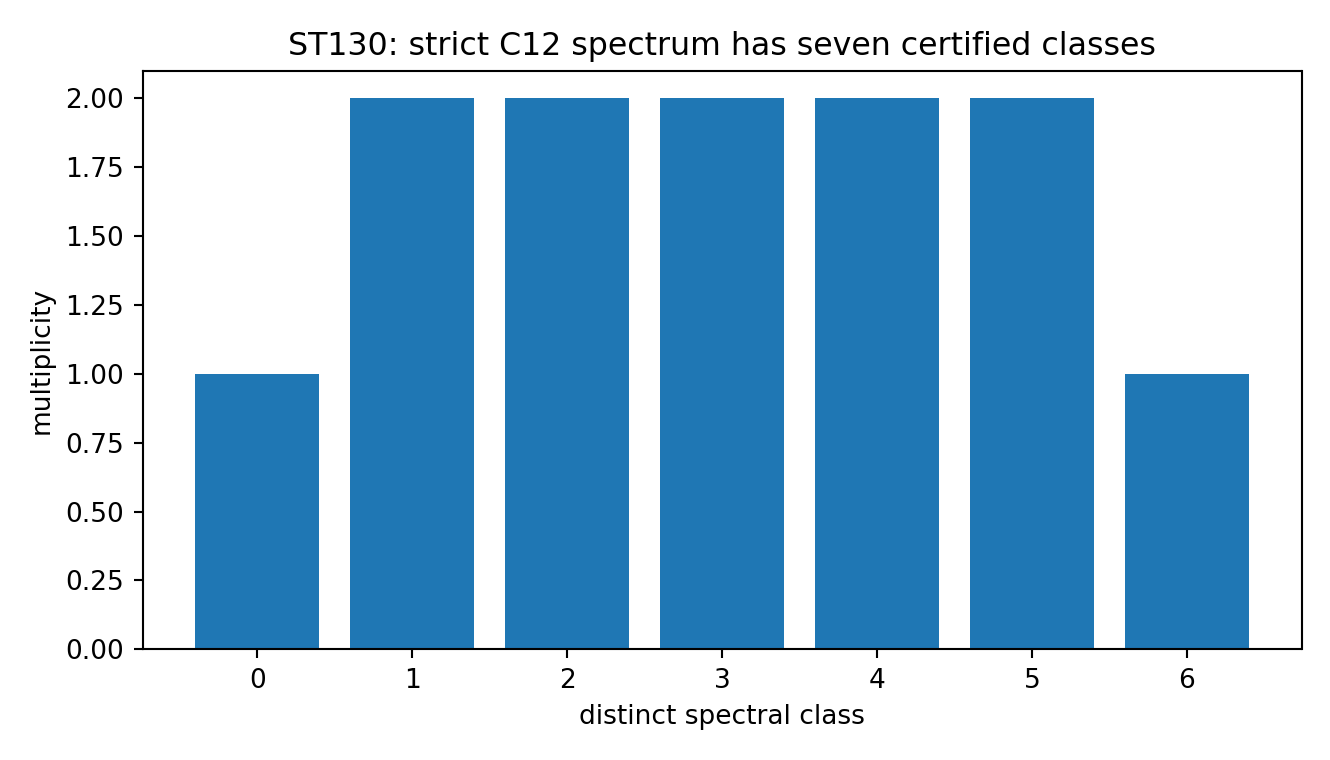
\includegraphics[width=.72\textwidth]{FIN_ST130_ST141_Figures/st130_algebra_dimensions.png}
\caption{ST130. Multiplicities of the seven interval-separated strict spectral classes. The full fine $U(12)$ gauge is not the strict dynamical symmetry group.}
\end{figure}

This is the precise negative answer requested by ST130, but only in the stated class. A state-dependent quotient, environment-induced superselection, dilation, preparation equivalence, or instrument-defined indistinguishability can evade it by adding structure. The theorem does not close QW-2191.

\section{ST131 and ST132: lift geometry and independent fold discovery}

\subsection{An exact noncirculant face}

The complete fine-block fiber satisfies
\[
B\succeq0,\qquad B_{ii}\ge A_{ii},\qquad A_{ij}\le B_{ij}\le-A_{ij}\quad(i\ne j).
\]
Fix every off-diagonal entry at the lower endpoint. The resulting exposed face is
\[
\mathcal F_{\rm diag}=\{A+\operatorname{Diag}(t):t\in\mathbb R_+^{12}\}.
\]

\begin{theorem}[Orthant face and rank jump]
$\mathcal F_{\rm diag}$ is affinely a twelve-dimensional nonnegative orthant. It has $2^{12}=4096$ faces, one vertex $A$, and twelve extreme rays $E_{ii}$. The vertex has rank eleven; every point with $t\ne0$ is positive definite and has rank twelve.
\end{theorem}

\textit{Proof.} The coordinate constraints expose the orthant. If
$x^*(A+\operatorname{Diag}(t))x=0$, both nonnegative terms vanish. Connectivity of the positive-weight strict graph makes $x$ constant, while any positive $t_i$ forces that constant to vanish. \hfill$\square$

Thus ST131 falsifies the hoped-for nontrivial low-rank continuation on this natural noncirculant face. It does not classify the remaining bounded faces of the 78-dimensional spectrahedron.

\subsection{The fold center is no longer imported}

ST132 starts from the deliberately coarse localized ansatz
\[
q=(2.5,.2,.08,.03,.015,.008,.004),\quad \kappa=.02,
\quad v=(0,-1,0,0,0,0,0).
\]
No ST108 or ST120 result file is opened. Four damped-Newton steps produce the fold center with residual
\[
\|G(x_*)\|_\infty=6.94\times10^{-17}.
\]
The independently rebuilt interval system then gives strict Krawczyk inclusion in the radius-$10^{-8}$ box, with margin
\[
9.999987060638205\times10^{-9}.
\]

\begin{figure}[H]\centering
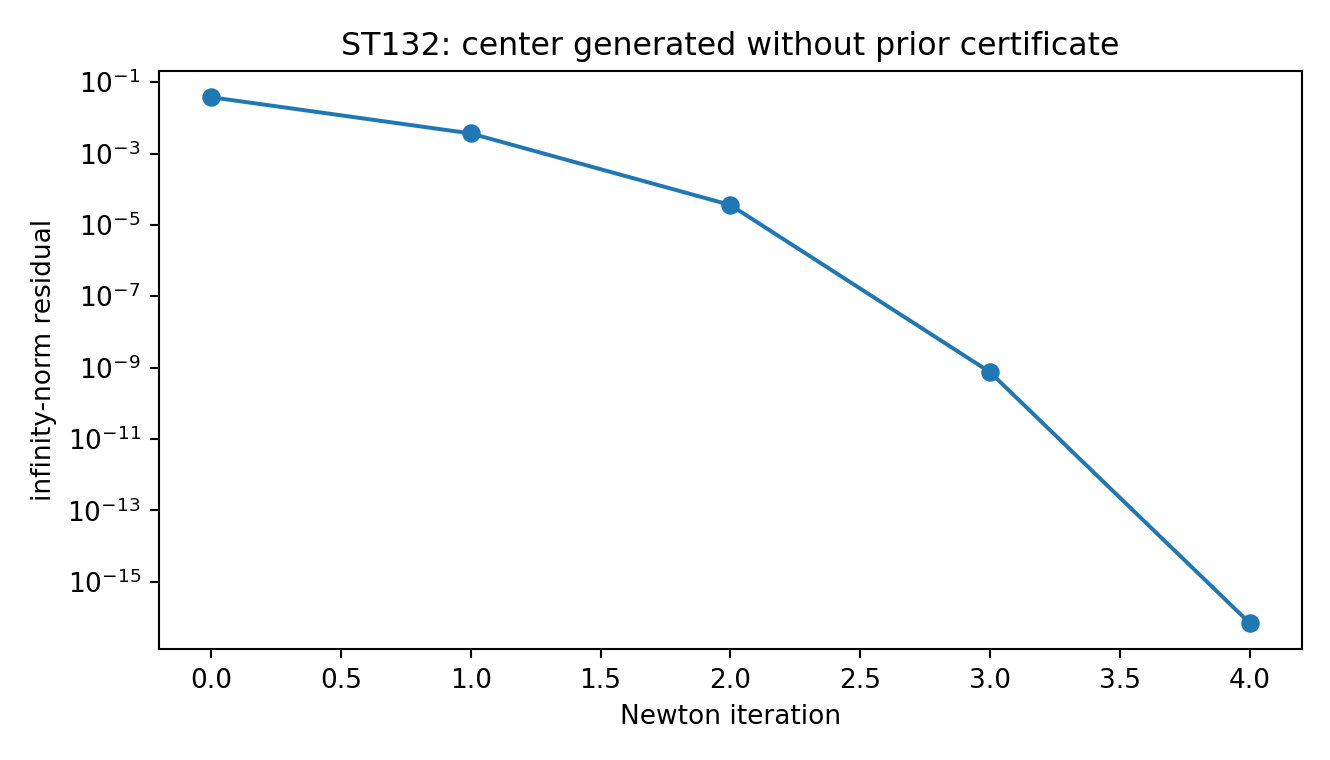
\includegraphics[width=.72\textwidth]{FIN_ST130_ST141_Figures/st132_center_isolation.png}
\caption{ST132. Residual decay from the coarse localized seed; the final root is certified separately by interval inclusion.}
\end{figure}

\proven{} There is exactly one root in the certified local box for every strict operator enclosed by the declared transcendental interval evaluation. \statusboundary{} The coarse ansatz still selects a basin, and no exhaustive compact-domain root count has been proved.

\section{ST133 and ST134: noisy recovery and the cost of a selector state}

\subsection{Optimal recovery under a declared noisy pinching channel}

Let $\Pi_{cf}$ be coarse/fine pinching and let $\mathcal D_{24}(X)=\operatorname{Tr}(X)I_{24}/24$. The declared channel is
\[
\mathcal N_\varepsilon=(1-\varepsilon)\Pi_{cf}+\varepsilon\mathcal D_{24}.
\]
For every maximal graph code classified in ST121, the sector recovery converts it to
\[
\mathcal R\mathcal N_\varepsilon\mathcal V
=(1-\varepsilon)\operatorname{Id}_{12}+\varepsilon\mathcal D_{12}.
\]

\begin{theorem}[Optimal noisy-pinch recovery]
The maximum entanglement and average fidelities are
\[
F_e^*=1-\varepsilon+\frac{\varepsilon}{144},
\qquad
F_{\rm av}^*=1-\frac{11}{12}\varepsilon.
\]
\end{theorem}

The pinching branch is exactly recoverable. The depolarizing branch contains no input information and no recovery can exceed $1/144$ entanglement fidelity there. The same recovery attains both branch optima.

\begin{figure}[H]\centering
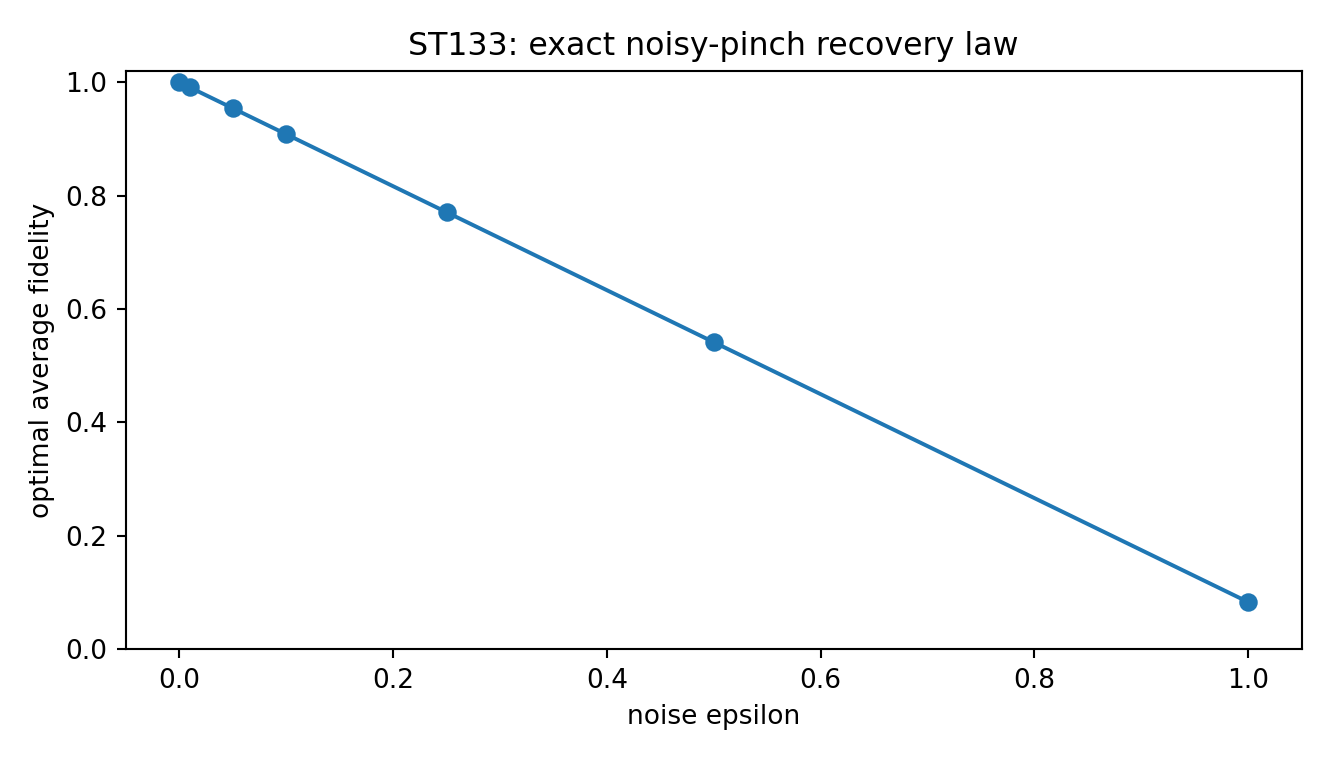
\includegraphics[width=.72\textwidth]{FIN_ST130_ST141_Figures/st133_noisy_recovery.png}
\caption{ST133. Exact optimal average fidelity for the declared depolarizing-pinch model.}
\end{figure}

\subsection{No positive selector cost without preparation constraints}

Consider
\[
\rho_\varepsilon=(1-\varepsilon)\frac I{12}+\varepsilon|0\rangle\!\langle0|,
\qquad \varepsilon>0.
\]
Every member has a unique preferred vertex. At $\varepsilon=1$ it is rank one, which is the minimum possible nonzero density rank. Its cyclic twirl is $I/12$, and the pure-state asymmetry costs are
\[
\frac12\bigl\||0\rangle\!\langle0|-I/12\bigr\|_1=\frac{11}{12},
\qquad D(|0\rangle\!\langle0|\|I/12)=\ln12.
\]

\begin{theorem}[Vanishing selector-cost infimum]
Over all noninvariant density states, the infimum of both trace-distance-to-twirl and relative-entropy asymmetry is zero, even when the diagonal record has a unique maximizer.
\end{theorem}

The proof is the family $\rho_\varepsilon$ as $\varepsilon\downarrow0$. Therefore state-space geometry alone cannot assign a positive minimum cost to symmetry breaking.

\begin{figure}[H]\centering
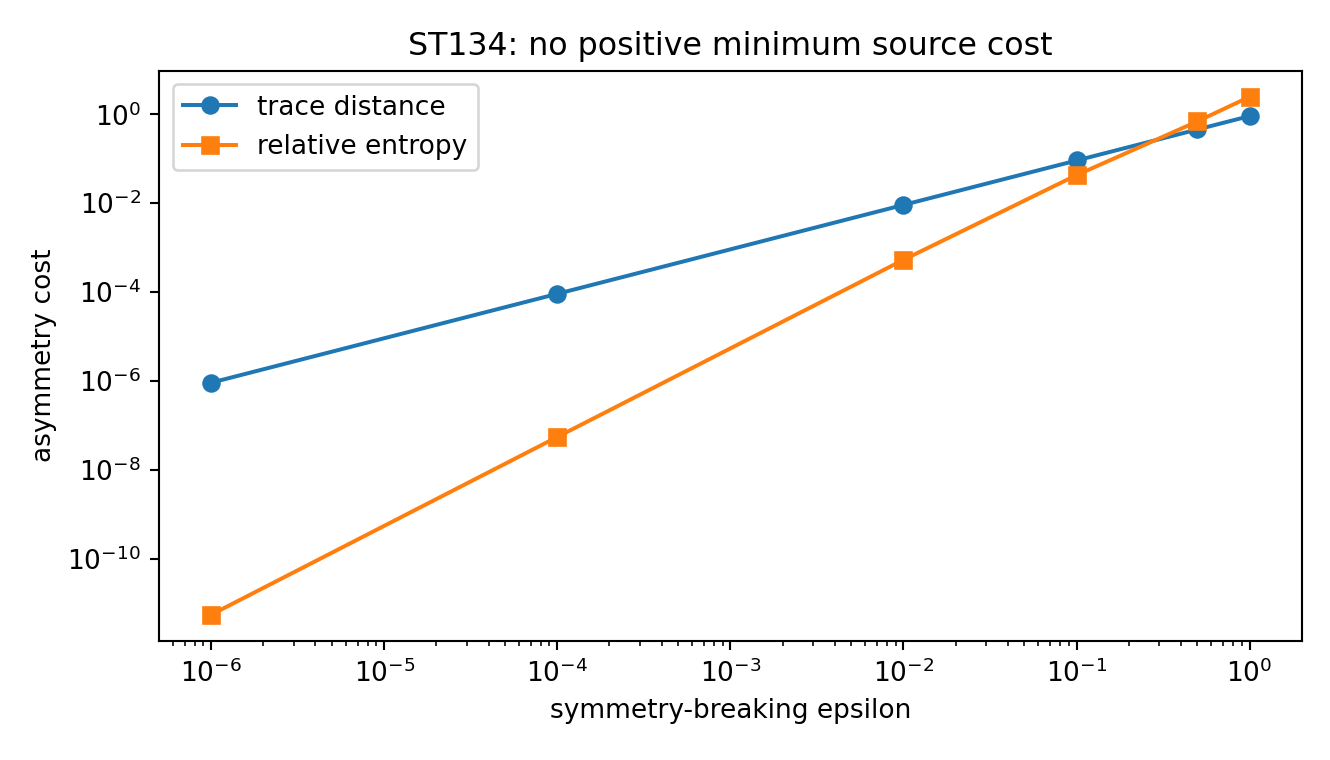
\includegraphics[width=.72\textwidth]{FIN_ST130_ST141_Figures/st134_asymmetry_cost.png}
\caption{ST134. A unique preferred branch persists for every $\varepsilon>0$, while both asymmetry resources vanish continuously.}
\end{figure}

This turns the selector question into a sharper one: which preparation constraints, finite resolution, action budget, or robustness requirement could enforce a nonzero operational cost? The displayed state is supplied and does not discharge QW-2191.

\section{ST135 and ST136: pumped strict modes and robust local design}

\subsection{What a minimal pumped modal extension actually selects}

On a strict eigenspace of eigenvalue $\lambda_r$, define the constructed dynamics
\begin{equation}
\dot z=\left(g-\gamma-\nu\lambda_r+i\lambda_r\right)z-\kappa\|z\|^2z,
\qquad \kappa>0.
\label{eq:pumpedmode}
\end{equation}
Write $\mu_r=g-\gamma-\nu\lambda_r$.

\begin{theorem}[Modal orbital stability]
For $\mu_r\le0$, $z=0$ is stable. For $\mu_r>0$, the orbit
\[
\|z\|=\sqrt{\mu_r/\kappa}
\]
is radially attracting with exponent $-2\mu_r$ and has neutral phase and eigenspace tangents.
\end{theorem}

After removal of the constant mode, the first instability occurs in a twofold strict eigenspace. It produces a degenerate attracting orbit, not a unique orientation or localized soliton.

\begin{figure}[H]\centering
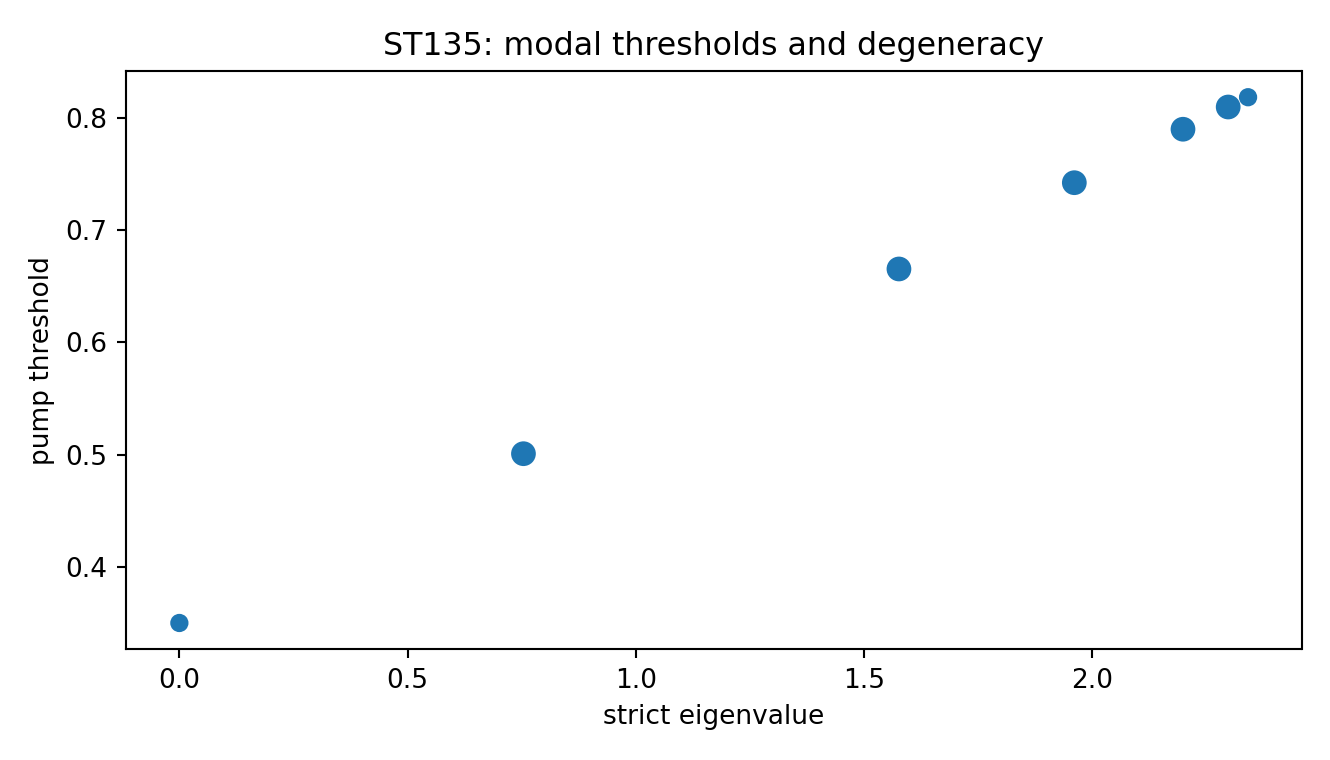
\includegraphics[width=.72\textwidth]{FIN_ST130_ST141_Figures/st135_mode_thresholds.png}
\caption{ST135. Pump thresholds $g_r=\gamma+\nu\lambda_r$; marker area records spectral multiplicity.}
\end{figure}

The model makes the earlier symmetry/feedback distinction exact. Symmetry supplies degeneracy; the pump creates instability; saturation bounds amplitude. The pump, loss, clock, nonlinearity, and modal decoupling are not strict-derived.

\subsection{Parametric interval design}

ST136 promotes the nominal stationary Chernoff root to a uniform local result over
\[
q_0\in[0.19999,0.20001],\quad q_1\in[0.69999,0.70001],\quad
\delta\in[0.04999,0.05001].
\]
The nominal center is
\[
(\beta_*,\sigma_*)=(2.186189925005267,0.539833703306342).
\]
A rectangular root box with radii $(0.003,0.008)$ has strict Krawczyk inclusion margin
\[
0.0018927591441788572.
\]

\proven{} For every nuisance triple in the displayed box, there is exactly one stationary root in the common rectangular state box. The proof uses outward-enclosed frozen binary64 spectra. It neither proves that the stationary point is the global $\beta$ optimum nor supplies physical inverse temperature or detector calibration.

\section{ST137 and ST138: refinement cohomology and causal nonselection}

\subsection{All finite twisted refinements reduce to affine transport}

Write $h=(-1)^x$ with $x\in\mathbb F_2$. A degree-$m$ edge with twist $\tau$ acts as
\[
x_{\rm out}=(m\bmod2)x_{\rm in}+\tau.
\]
Represent it by an affine pair $(a,b)$. Composition is
\[
(a_2,b_2)\circ(a_1,b_1)=(a_2a_1,a_2b_1+b_2).
\]

\begin{theorem}[Path-independent twist criterion]
A twist assignment on any finite refinement diagram is coherent exactly when all parallel paths have the same composite affine pair. If two paths have different products of degree parity, no twists can make them equal for both input holonomies. If the parity products agree, coherence is a linear cocycle system over $\mathbb F_2$.
\end{theorem}

Exhaustive four-edge diamond tests give $8/16$ coherent twist assignments when both path parities agree and $0/16$ when they disagree. This is a general algorithmic criterion, not a source of the degrees or twists.

\subsection{Conditional independence does not name its conditioning algebra}

In $M_2\otimes M_2$ with normalized trace, consider
\[
E_1=\operatorname{id}\otimes\tau,
\qquad E_2=\tau\otimes\operatorname{id}.
\]
Both are faithful trace-preserving conditional expectations and obey the same product-state conditional-independence and commuting-square identities. Their ranges are distinct: $M_2\otimes I$ and $I\otimes M_2$.

\begin{theorem}[Untyped causal-independence nonselection]
Abstract conditional-independence identities cannot uniquely select their own conditioning algebra. A region net, subsystem assignment, accessible instrument class, or equivalent operational typing is necessary.
\end{theorem}

Unitary conjugation yields a continuum of further examples. Thus causality language alone does not repair ST130; a genuinely typed causal net might, but would be additional structure.

\section{ST139: positive count exponents require quantified dependence}

ST127 showed that arbitrary temporal correlation can reduce every $n$-event record to one bit. ST139 supplies a positive counterpart. Divide $n=km$ detector events into known blocks of length $m=5$. Events within a block are identical; blocks are independent. Under the two hypotheses, the block bit has probabilities $p_0=.72$ and $p_1=.94$.

\begin{theorem}[Exact finite-range count law]
The complete raw record is statistically equivalent to $k$ independent Bernoulli observations. Its equal-prior Bayes error is
\[
P_e(k)=\frac12\sum_{j=0}^{k}\min\left\{\binom kjp_0^j(1-p_0)^{k-j},
\binom kjp_1^j(1-p_1)^{k-j}\right\},
\]
and
\[
P_e(k)\le\frac12e^{-kC},\qquad C=0.04942597528209407.
\]
The exponent per raw event is $C/5=0.009885195056418813$.
\end{theorem}

\begin{figure}[H]\centering
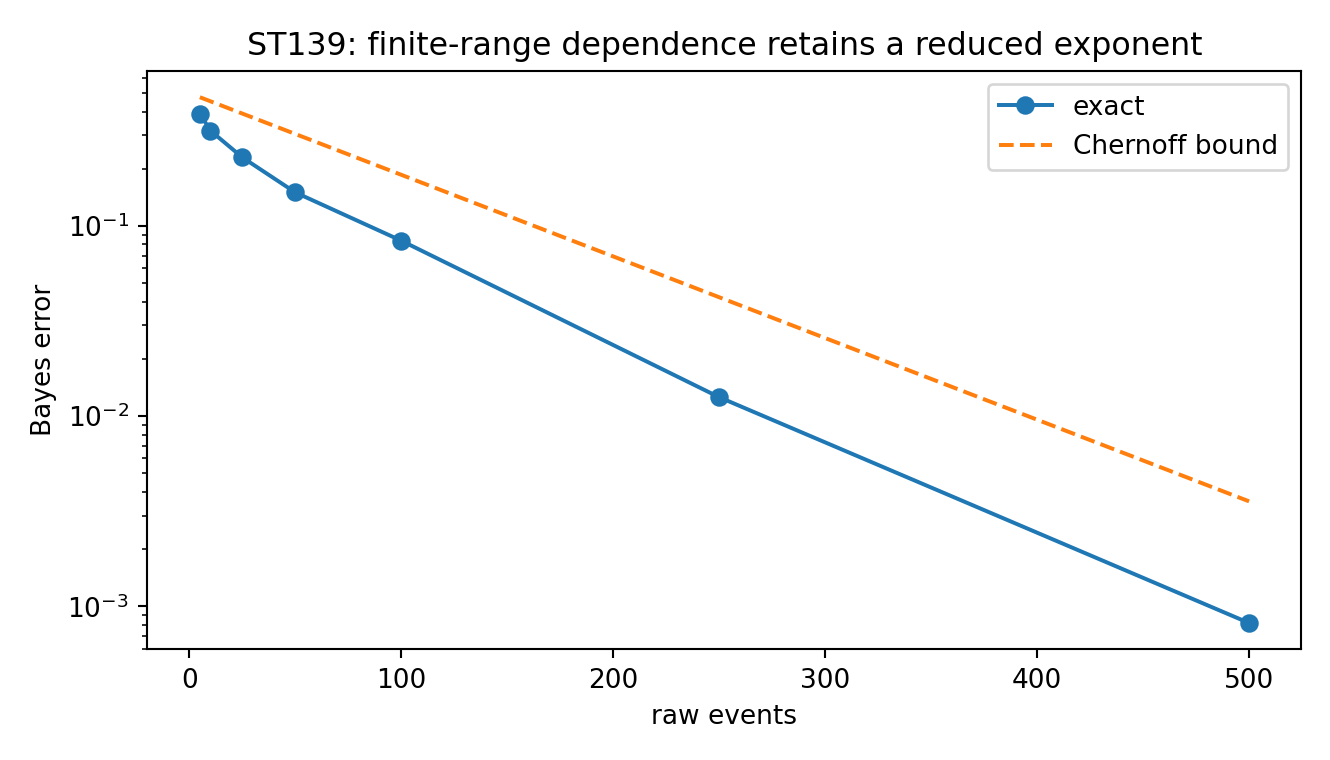
\includegraphics[width=.72\textwidth]{FIN_ST130_ST141_Figures/st139_dependent_counts.png}
\caption{ST139. Exact error and Chernoff upper bound under the declared finite dependence length.}
\end{figure}

The result proves that quantified finite-range dependence restores exponential discrimination, with an explicit penalty. It does not infer the block law or correlation length from FIN data.

\section{ST140: one energy-bearing bath qubit}

Choose two strict spectral vectors separated by the dimensionless gap
\[
\Delta=0.7541211542070796
\]
and a bath qubit with the same gap. At $\beta=.8$, its populations are
\[
b_0=0.6464102276045693,\qquad b_1=0.3535897723954306.
\]
An excitation-exchange unitary commutes exactly with $H_S+H_B$. For exchange angle $\theta$,
\[
p_{\uparrow}=b_1\sin^2\theta,qquad p_{\downarrow}=b_0\sin^2\theta,
\qquad \frac{p_\uparrow}{p_\downarrow}=e^{-\beta\Delta}.
\]

\begin{theorem}[Matched-gap dilation]
At $\theta=\pi/2$, the selected two-level subsystem is reset exactly to its Gibbs state. On the full twelve-level strict system, a single matched-gap qubit leaves all unaddressed spectral populations invariant and therefore cannot implement a global Gibbs reset.
\end{theorem}

\begin{figure}[H]\centering
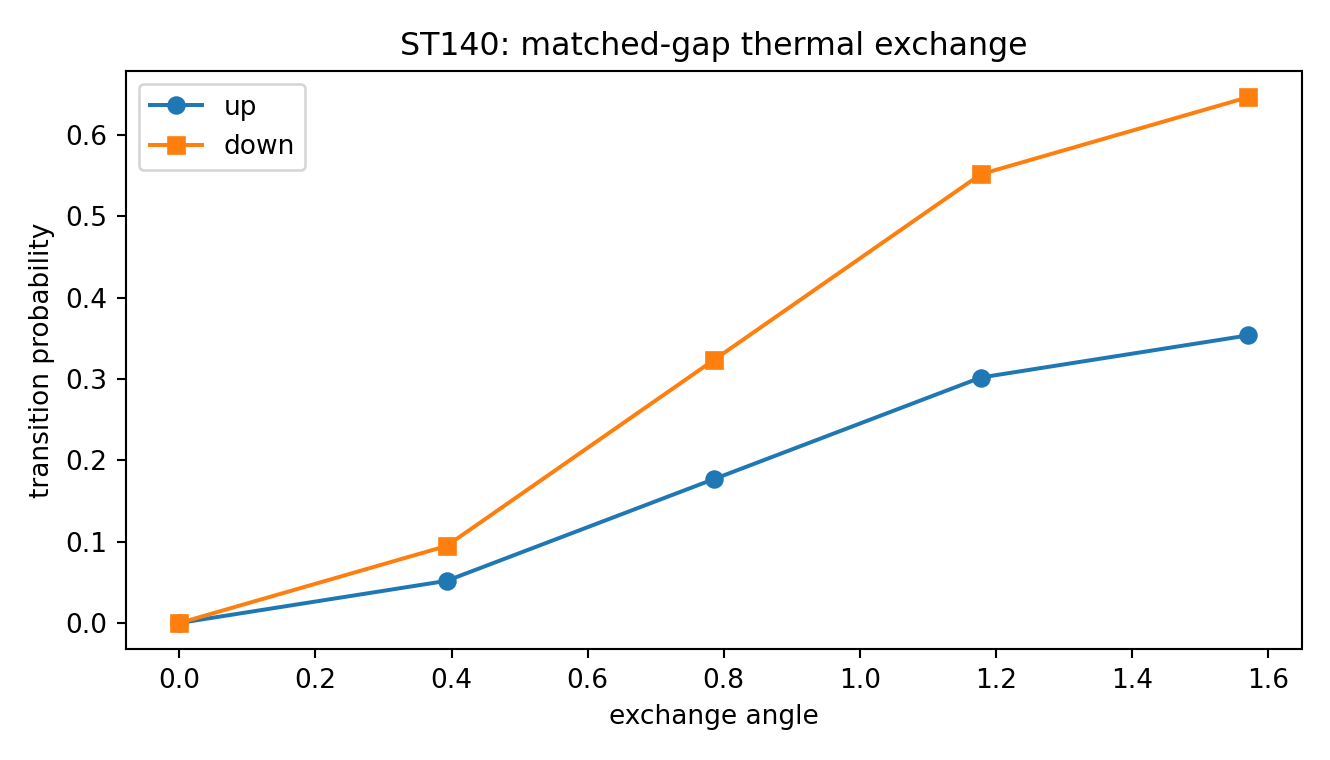
\includegraphics[width=.72\textwidth]{FIN_ST130_ST141_Figures/st140_matched_gap_bath.png}
\caption{ST140. Exact upward and downward transition probabilities under matched-gap exchange.}
\end{figure}

This goes beyond the zero-Hamiltonian bath class of ST128, but it remains a typed construction. The bath Hamiltonian, selected transition, $\beta$, interaction time, and interpretation of the dimensionless gap as energy all remain supplied.

\section{ST141: non-diagonal minimax observation}

Let $\Delta\succeq0$, $\operatorname{Tr}\Delta=1$, with entrywise nonnegative matrix entries. Then
\[
B=A+t\Delta
\]
remains graph-feasible for
\[
0\le t\le4\min_dw_d=0.04428326928576845.
\]
This bounded perturbation class contains every coordinate projector $E_{ii}$ and genuinely non-diagonal positive directions. Let $H\succeq0$, $\operatorname{Tr}H=1$ be a fine detector.

\begin{theorem}[Noisy non-diagonal minimax value]
\[
\max_H\min_\Delta\operatorname{Tr}(H\Delta)=\frac1{12}.
\]
The uniform detector $H_*=I/12$ attains the value. Under declared depolarizing measurement noise
\[
H\mapsto H_\delta=(1-\delta)H+\delta I/12,
\]
the minimax value remains $1/12$ for every $\delta\in[0,1]$. An independent worst additive response error $\epsilon$ reduces the certified guarantee to $\max(0,1/12-\epsilon)$.
\end{theorem}

\textit{Proof.} Since the adversary contains $E_{ii}$,
$\min_\Delta\operatorname{Tr}(H\Delta)\le\min_iH_{ii}\le\operatorname{Tr}H/12$. The uniform detector returns $1/12$ on every trace-one $\Delta$ and is fixed by the noise map. \hfill$\square$

\begin{figure}[H]\centering
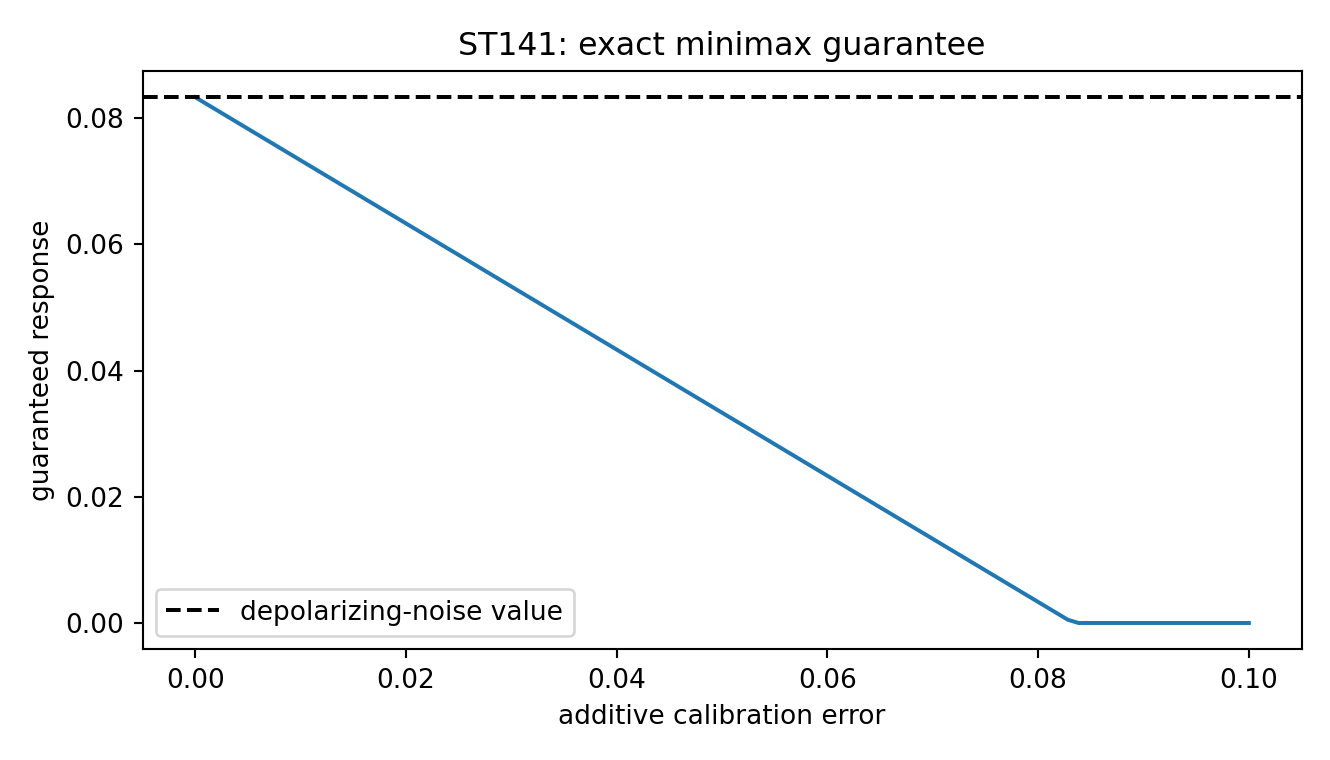
\includegraphics[width=.72\textwidth]{FIN_ST130_ST141_Figures/st141_minimax_noise.png}
\caption{ST141. Depolarizing measurement noise leaves the uniform minimax value fixed; adversarial additive calibration error lowers the guarantee linearly.}
\end{figure}

The theorem extends the diagonal simplex value of ST129 to a non-diagonal graph-feasible class. It does not prove uniqueness of all optimal detectors or construct a laboratory POVM.

\section{What survived falsification}

The batch separates four statements that had previously been easy to conflate:
\begin{enumerate}
\item \textbf{A gauge can define the projection, but strict functional calculus does not generate that gauge.}
\item \textbf{A noninvariant state can select a branch, but unconstrained state space assigns no positive minimum cost to doing so.}
\item \textbf{A pump can destabilize a symmetric state, but the first strict positive mode remains degenerate and does not select an orientation.}
\item \textbf{An energy-bearing bath can thermalize a selected transition, but a single matched gap cannot thermalize the full strict spectrum.}
\end{enumerate}

The deepest conclusion is therefore not a new physical law. It is an object-level diagnosis: an operational completion of FIN must contain at least a typed redundancy/equivalence, a constrained preparation resource, a dynamical symmetry-breaking source, and an environment with sufficient energy support. None is supplied by $A$ alone in the classes tested here.

\section{Recommended programs ST142--ST153}
\small
\begin{longtable}{@{}p{0.06\textwidth}p{0.48\textwidth}p{0.38\textwidth}@{}}
\toprule Priority & Program & Decisive output\\\midrule\endfirsthead
\toprule Priority & Program & Decisive output\\\midrule\endhead
1 & \textbf{ST142}: natural operational quotients beyond functional calculus & Source theorem or broader naturality no-go without pre-naming fine sector\\
2 & \textbf{ST143}: bounded noncirculant face adjacency & Certified face lattice beyond the diagonal orthant\\
3 & \textbf{ST144}: compact-domain multibasin fold isolation & Exhaustive root count or explicit missed roots\\
4 & \textbf{ST145}: coherent leakage and asymmetric misclassification & Optimal recovery channel and fidelity theorem\\
5 & \textbf{ST146}: preparation-constrained asymmetry & Positive source cost or impossibility theorem\\
6 & \textbf{ST147}: equivariant nonlinear coupling in first degenerate mode & Orbital stability and branch-orbit classification\\
7 & \textbf{ST148}: widen the ST136 nuisance box & Certified continuation boundary or first bifurcation\\
8 & \textbf{ST149}: arbitrary refinement DAG checker & Exact affine-cohomology certificate and counterexample output\\
9 & \textbf{ST150}: typed causal region net & Minimality theorem or persistent ST138 ambiguity\\
10 & \textbf{ST151}: stationary hidden-Markov detector drift & Finite-count bounds from certified contraction\\
11 & \textbf{ST152}: multi-gap bath ladder & Bath-dimension bounds for approximate global Gibbs reset\\
12 & \textbf{ST153}: all minimax detectors on the graph-feasible cone & Complete optimizer-face classification under noise\\
\bottomrule
\end{longtable}
\normalsize

The highest-priority conceptual program remains ST142. ST130 closes only the strict functional-calculus route; the scientifically honest next question is whether a larger but still natural operational category generates the equivalence, or whether every such construction necessarily imports the fine sector through its typing.

\section{Reproducibility}

The package contains:
\begin{itemize}
\item \texttt{fin\_st130\_st141\_research.py};
\item the standalone \texttt{fin\_st132\_center\_isolation\_replay.py};
\item \texttt{test\_fin\_st130\_st141.py} with 30 tests, including live recomputation;
\item the complete JSON ledger and CSV summary;
\item individual ST131, ST132, ST136, ST137, ST140, and ST141 certificates/packets;
\item eight generated figures and a SHA-256 manifest.
\end{itemize}

The main run uses Python 3.12, NumPy 1.26.4, SciPy 1.17.1, mpmath interval arithmetic, and Matplotlib. The standalone ST132 replay uses only NumPy and mpmath as third-party dependencies. The command
\[
\texttt{python3 -m unittest -v test\_fin\_st130\_st141.py}
\]
passes all 30 tests. Live tests reconstruct the spectral obstruction, rank jump, fold isolation, fidelity formulas, rectangular parametric inclusion, refinement counts, finite-count bounds, energy conservation, detailed balance, and graph feasibility.

\section{Final verdict}

\resultbox{\textbf{Verdict surviving ST130--ST141.} The strict spectral operator remains a coherent generator of multiple mathematical channels, but it does not generate the operational fine gauge in the tested natural class. A selector state can be arbitrarily close to symmetric, a pump leaves a degenerate mode orbit, conditional independence does not identify its own algebra, and one matched-gap bath addresses only one transition. The next missing theorem must therefore concern a typed operational category and constrained resources, not another relabeling of $f(A)$.}

No strict fine-gauge source, QW-2191 discharge, dimensional clock or unit, preparation apparatus, independent laboratory record, legacy-to-strict completion or role transfer, Standard Model, gravity, $L_{\rm total}$, physical projection theorem, or Theory-of-Everything closure is claimed.

\begin{thebibliography}{9}
\bibitem{BratteliRobinson} O. Bratteli and D. W. Robinson, \emph{Operator Algebras and Quantum Statistical Mechanics I}, Springer, 2nd ed., 1987.
\bibitem{Krawczyk} R. Krawczyk, ``Newton-Algorithmen zur Bestimmung von Nullstellen mit Fehlerschranken,'' \emph{Computing} 4 (1969), 187--201.
\bibitem{KnillLaflamme} E. Knill and R. Laflamme, ``Theory of quantum error-correcting codes,'' \emph{Physical Review A} 55 (1997), 900--911.
\bibitem{GourSpekkens} G. Gour and R. W. Spekkens, ``The resource theory of quantum reference frames: manipulations and monotones,'' \emph{New Journal of Physics} 10 (2008), 033023.
\bibitem{Chernoff} H. Chernoff, ``A measure of asymptotic efficiency for tests of a hypothesis based on the sum of observations,'' \emph{Annals of Mathematical Statistics} 23 (1952), 493--507.
\bibitem{HorodeckiOppenheim} M. Horodecki and J. Oppenheim, ``Fundamental limitations for quantum and nanoscale thermodynamics,'' \emph{Nature Communications} 4 (2013), 2059.
\end{thebibliography}

\end{document}
